\documentclass[a4paper,12pt]{article}

% --- Pacchetti Fondamentali ---
\usepackage[utf8]{inputenc} % Codifica caratteri
\usepackage[T1]{fontenc}    % Codifica font
\usepackage[italian]{babel} % Lingua italiana
\usepackage{geometry}       % Gestione margini
\usepackage{csquotes}      % Raccomandato da biblatex con babel/polyglossia
\usepackage{parskip}        % Gestione spazi tra paragrafi

\geometry{a4paper, margin=2.5cm}

% --- Pacchetti Matematica e Fisica ---
\usepackage{amsmath, amssymb} % Simboli matematici
\usepackage{siunitx}          % Gestione unità di misura e numeri (FONDAMENTALE)
\sisetup{
    output-decimal-marker = {.}, % Punto come separatore decimale
    separate-uncertainty = true, % Scrive errori come (Valore +/- Errore)
    per-mode = power,            % Usa / per le unità (m/s)
    inter-unit-product = \ensuremath{\cdot} % Per scrivere le unità con il punto (N·m)
}

% --- Pacchetti Immagini e Tabelle ---
\usepackage{graphicx} % Per inserire PNG/JPG
\usepackage{float}    % Per forzare la posizione delle immagini (H)
\usepackage{booktabs} % Per tabelle professionali (\toprule, \midrule)
\usepackage{caption}  % Per personalizzare le didascalie
\usepackage{subcaption}
\usepackage[font=small, labelfont=bf]{caption}
\usepackage[font=small, labelfont=bf]{subcaption}

% --- Dati Intestazione ---
\title{\textbf{Spettroscopia gamma}}
\author{Filippo Audisio, Cataldo Insalaco, Telemaco Pezzoni}
\date{\today}

\begin{document}

\maketitle

% -------------------------------------------------------------------

\section{Obiettivo dell'esperienza}
L'obiettivo dell'esperienza è caratterizzare lo spettro emesso da alcuni radionuclidi emettitori di radiazione gamma di energia nota, così da poter costruire una curva di calibrazione energetica. In particolare si vuole:
\begin{itemize}
    \item Acquisire lo spettro di: \texttt{Na-22}, \texttt{Ba-133}, \texttt{Cs-137}, \texttt{Am-241}.
    \item Costruire la curva di calibrazione energetica.
    \item Verificare la risoluzione del foto-rivelatore.
\end{itemize}

% -------------------------------------------------------------------
\section{Materiali e Metodi}

\subsection{Dotazione sperimentale}
\begin{itemize}
    \item Sorgenti radioattive: \texttt{Na-22}, \texttt{Ba-133}, \texttt{Cs-137}, \texttt{Am-241}.
    \item Rivelatore a scintillazione inorganico LaBr3 (Cs), accoppiato a un SiPM.
    \item Alimentatori per SiPM.
    \item Oscilloscopio.
    \item Amplificatore e digitalizzatore del segnale.
    \item Software Maestro.
    \item Blocco di Piombo.
\end{itemize}

\subsection{Procedura sperimentale}
Per prima cosa si accende il foto-rivelatore, alimentandoli con tensione predefinita, e si verifica la presenza di segnale dall'oscilloscopio avvicinando una sorgente al cristallo. Dopodiché si collega l'intera catena elettronica
per l'amplificazione e digitalizzazione del segnale e sfruttando il software Maestro si acquisisce lo spettro di ciascuna sorgente posizionandola sopra il rivelatore coperto da un panno, così da bloccare la luce ambientale. L'acquisizione per ogni sorgente viene effettuata per un  $\sim 10$ \unit{min}, mentre tra una misura e l'altra viene effettuata un'acquisizione di fondo per un tempo complessivo di $\sim 15$ \unit{min}. 
Infine per il Cs-137 si è effettuata una seconda acquisizione con un blocco di piombo posizionato sopra la sorgente, così da evidenziare il picco di backscattering.
% -------------------------------------------------------------------
\section{Dati sperimentali e Analisi}
\subsection{Spettri}
Dopo aver sottratto il fondo da ogni spettro, sono stati identificati i picchi corrispondenti alle energie note e nell'intorno di ciascun picco è stato eseguito un fit gaussiano, così da ricavare con maggiore precisione la posizione del picco stesso.
Per il fit è stata utilizzata la funzione:
\begin{equation}
    f(x) = a \cdot \exp\left(-\frac{(x-\mu)^2}{2\sigma^2}\right) + b 
\end{equation}

\begin{figure}[H]
     \centering
     \begin{subfigure}[b]{0.45\textwidth}
         \centering
         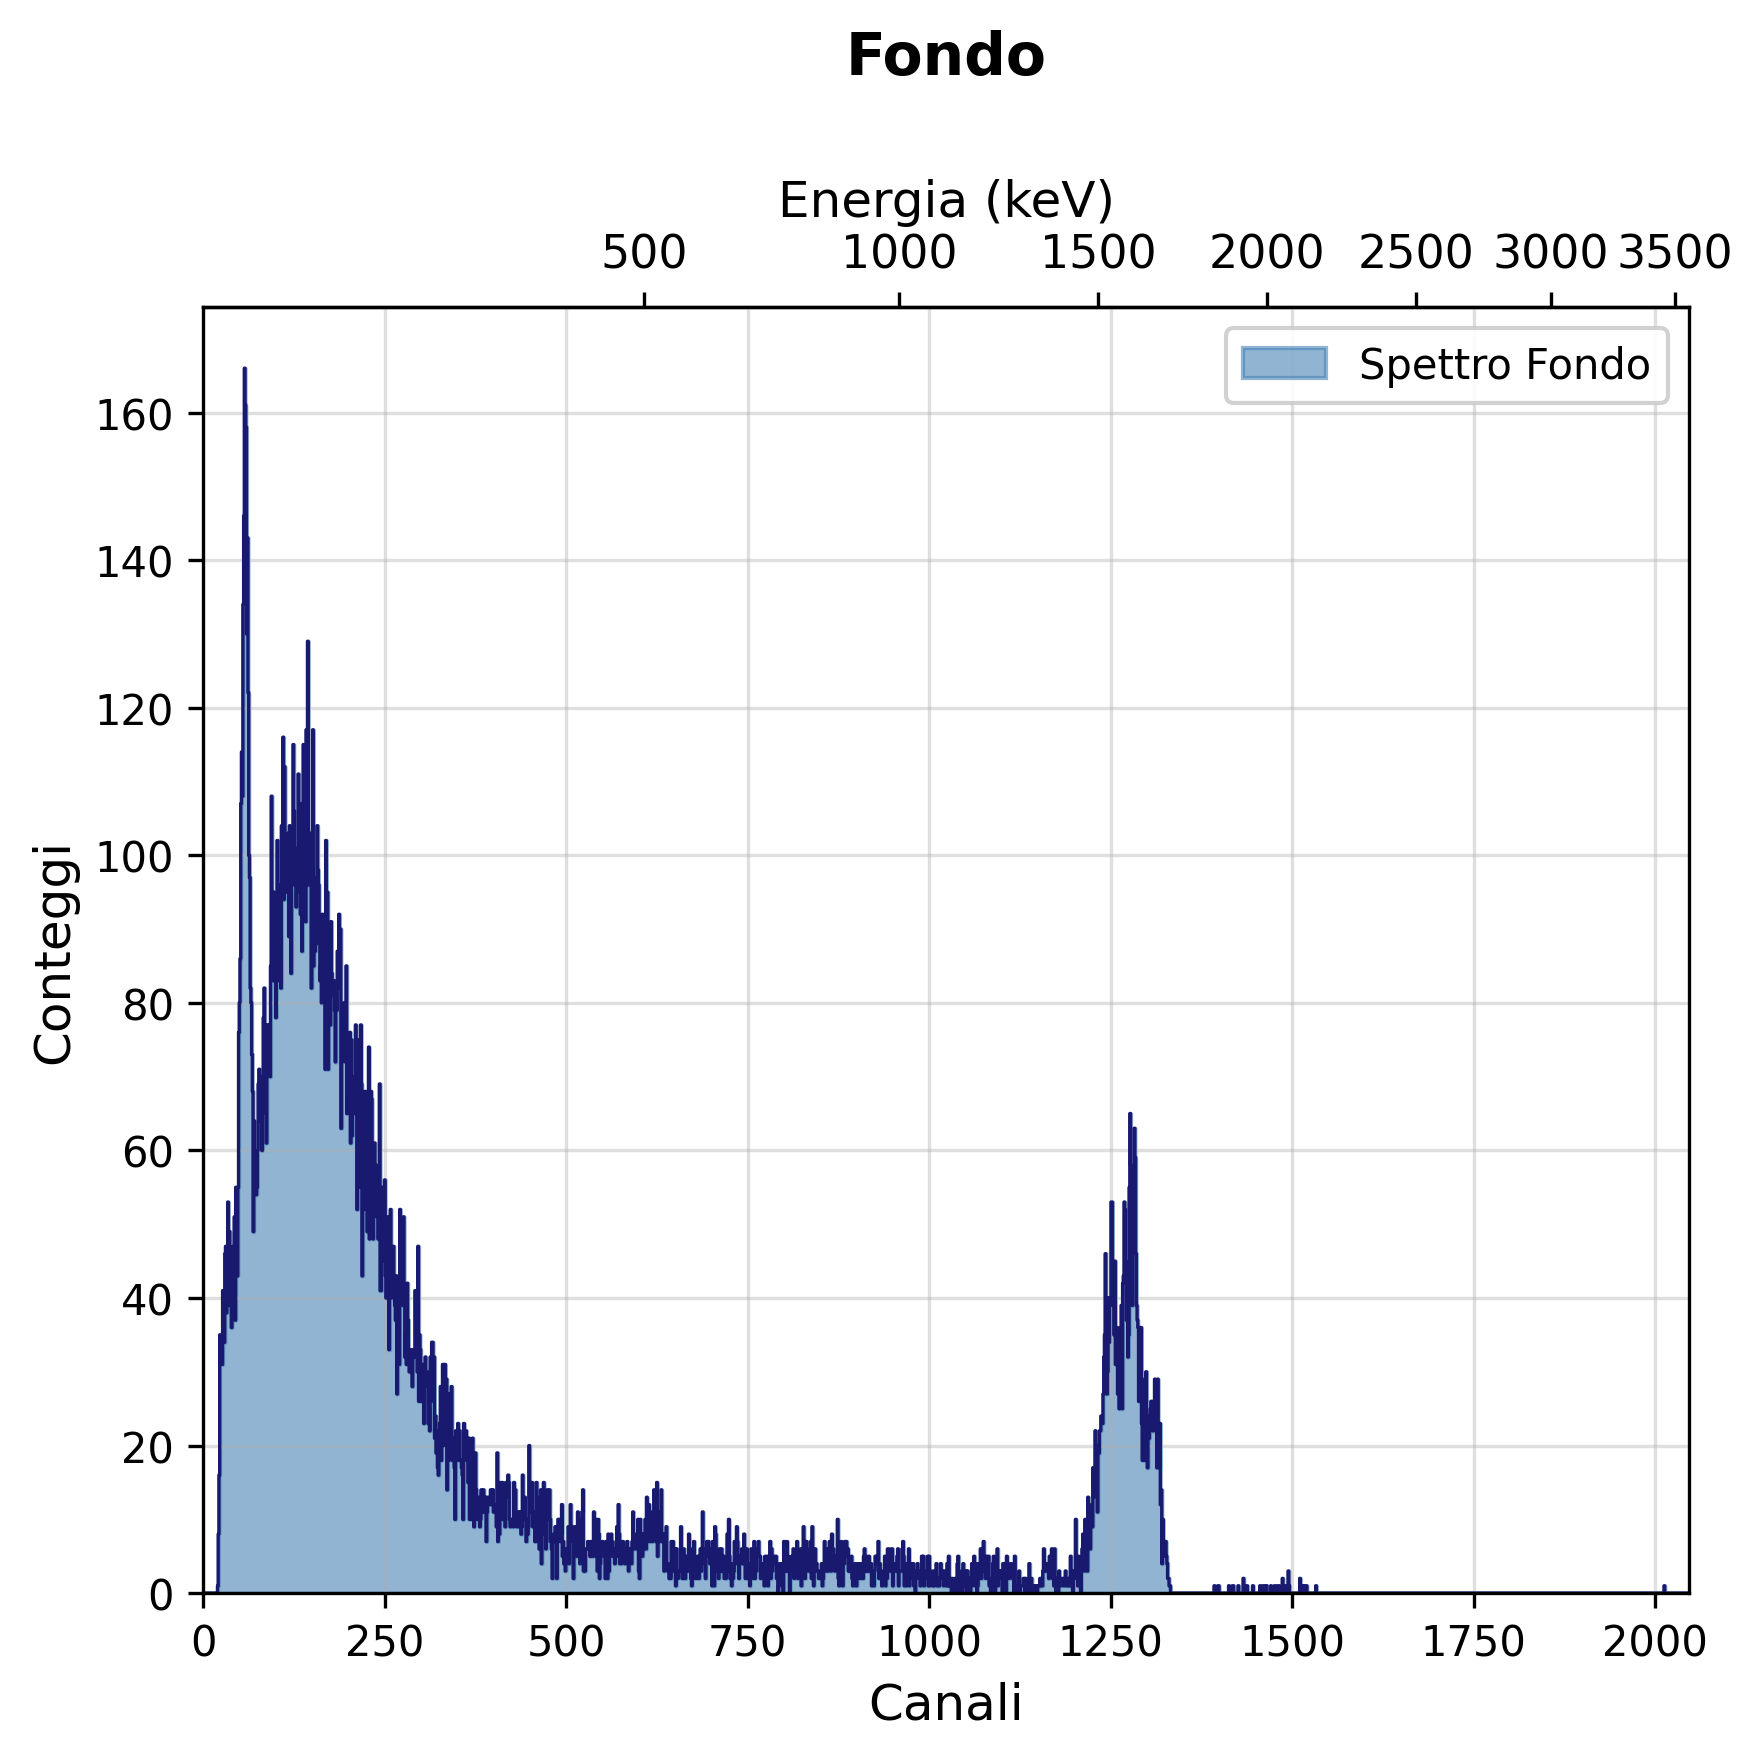
\includegraphics[width=\textwidth]{Spettro_Intero_Calibrato_Fondo.png}
         \label{fig:1a}
     \end{subfigure}
     \begin{subfigure}[b]{0.45\textwidth}
         \centering
         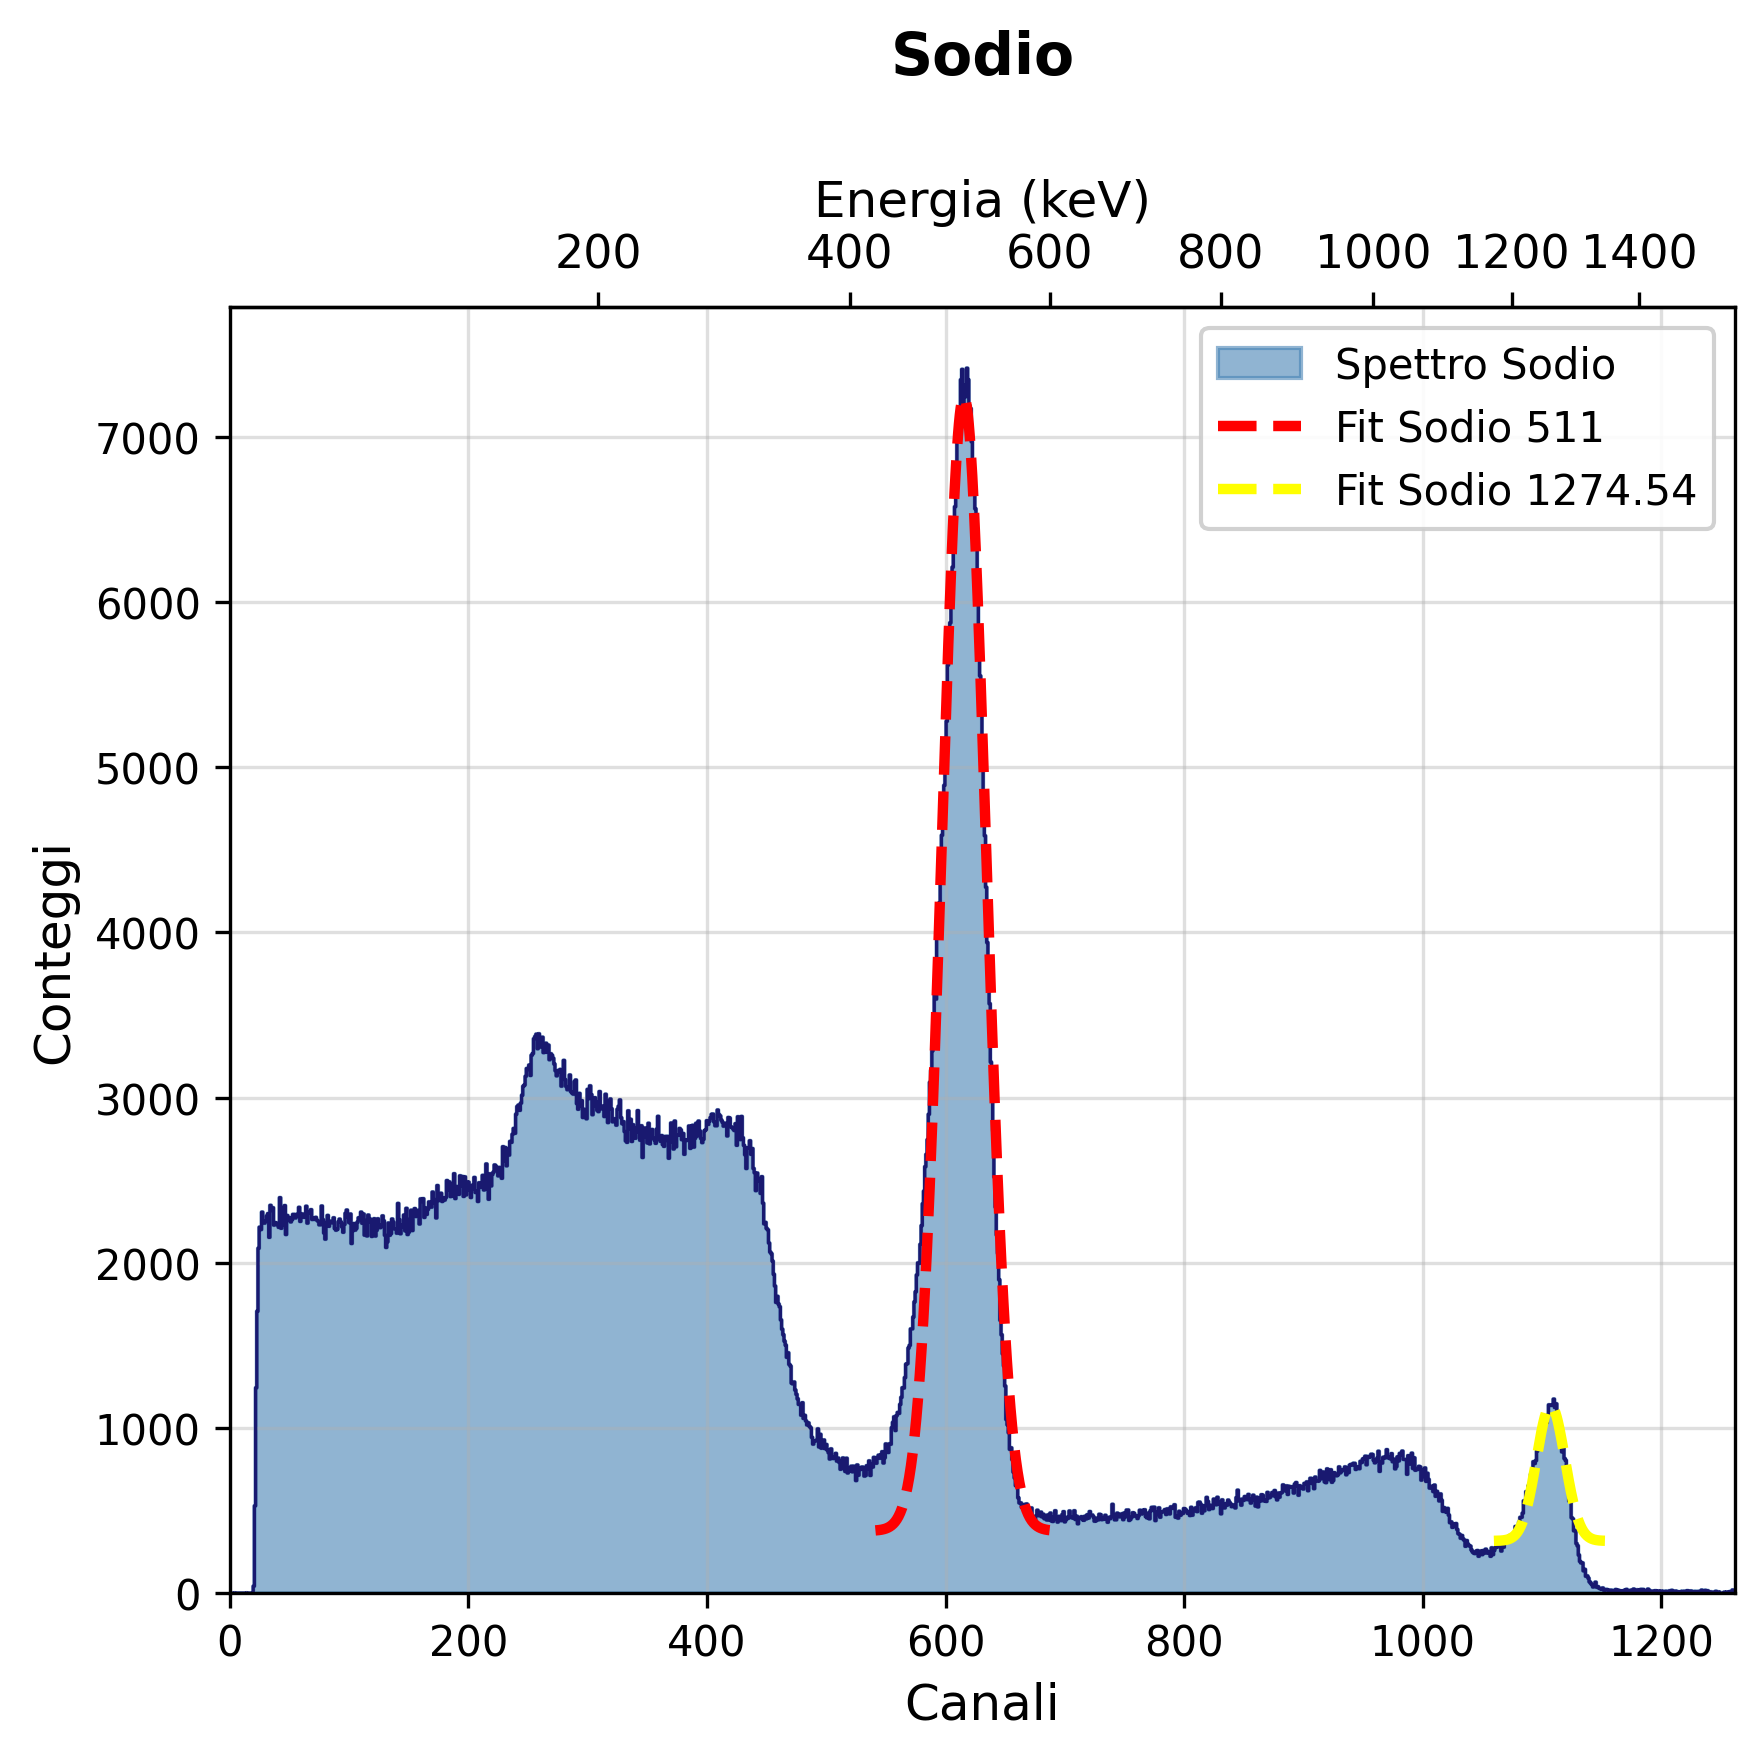
\includegraphics[width=\textwidth]{Spettro_Intero_Calibrato_Sodio.png}
         \label{fig:1b}
     \end{subfigure}
     \begin{subfigure}[b]{0.45\textwidth}
         \centering
         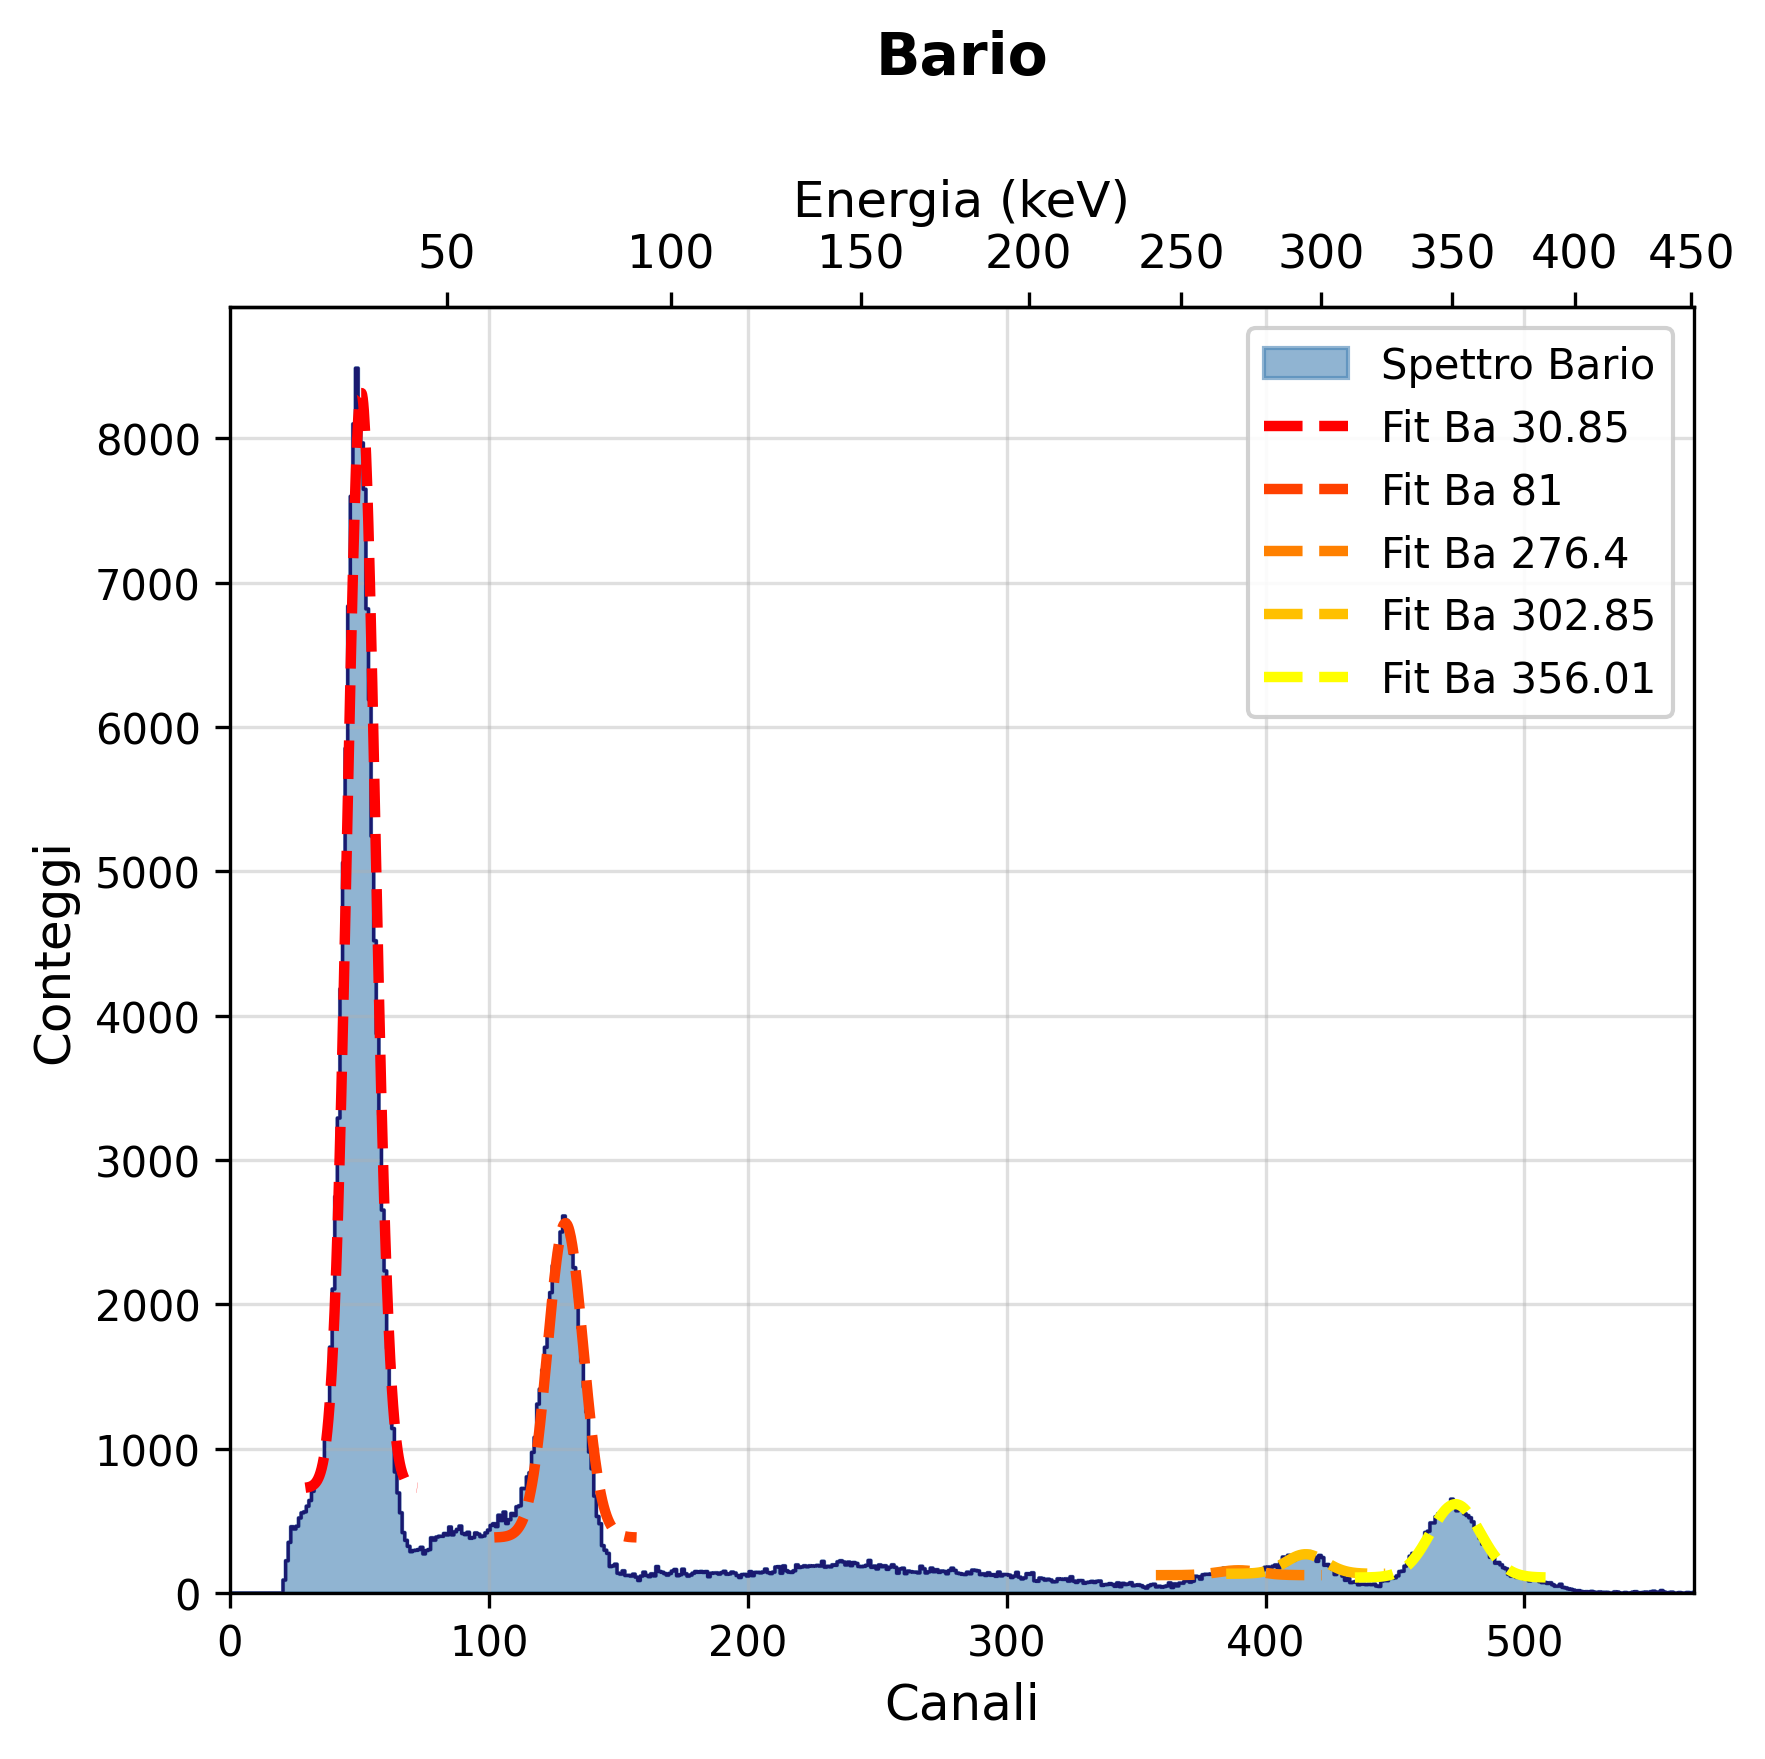
\includegraphics[width=\textwidth]{Spettro_Intero_Calibrato_Bario.png}
         \label{fig:1c}
     \end{subfigure}
     \begin{subfigure}[b]{0.45\textwidth}
         \centering
         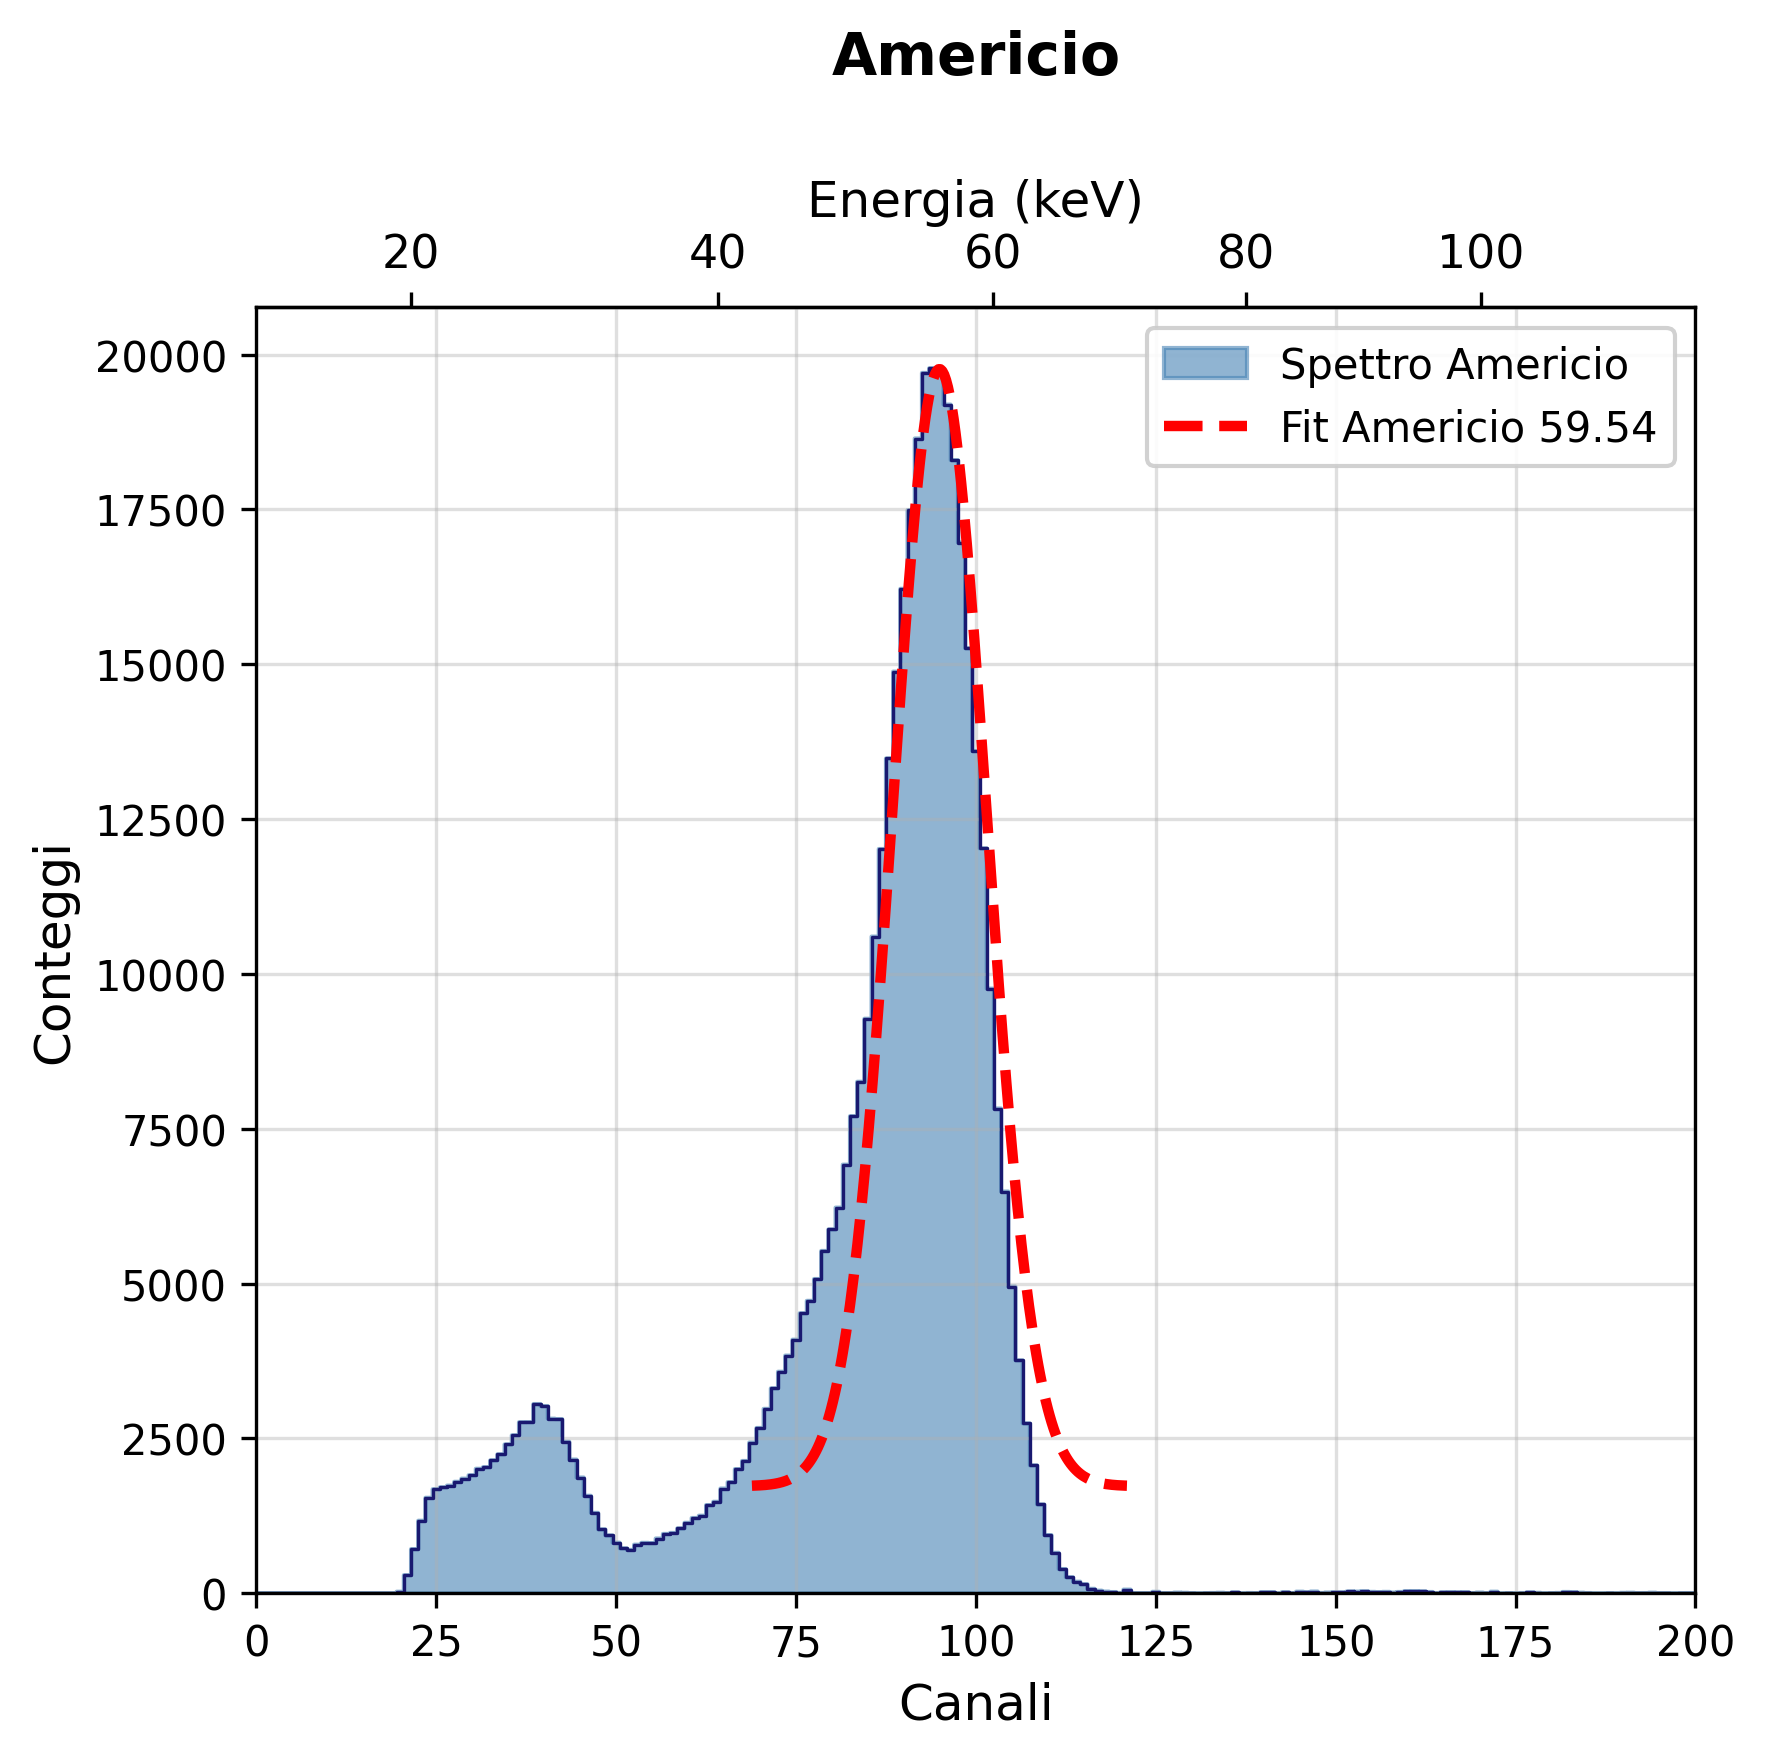
\includegraphics[width=\textwidth]{Spettro_Intero_Calibrato_Americio.png}
         \label{fig:1d}
     \end{subfigure}
\end{figure}

\begin{figure}[H]
     \centering
     \begin{subfigure}[b]{0.45\textwidth}
         \centering
         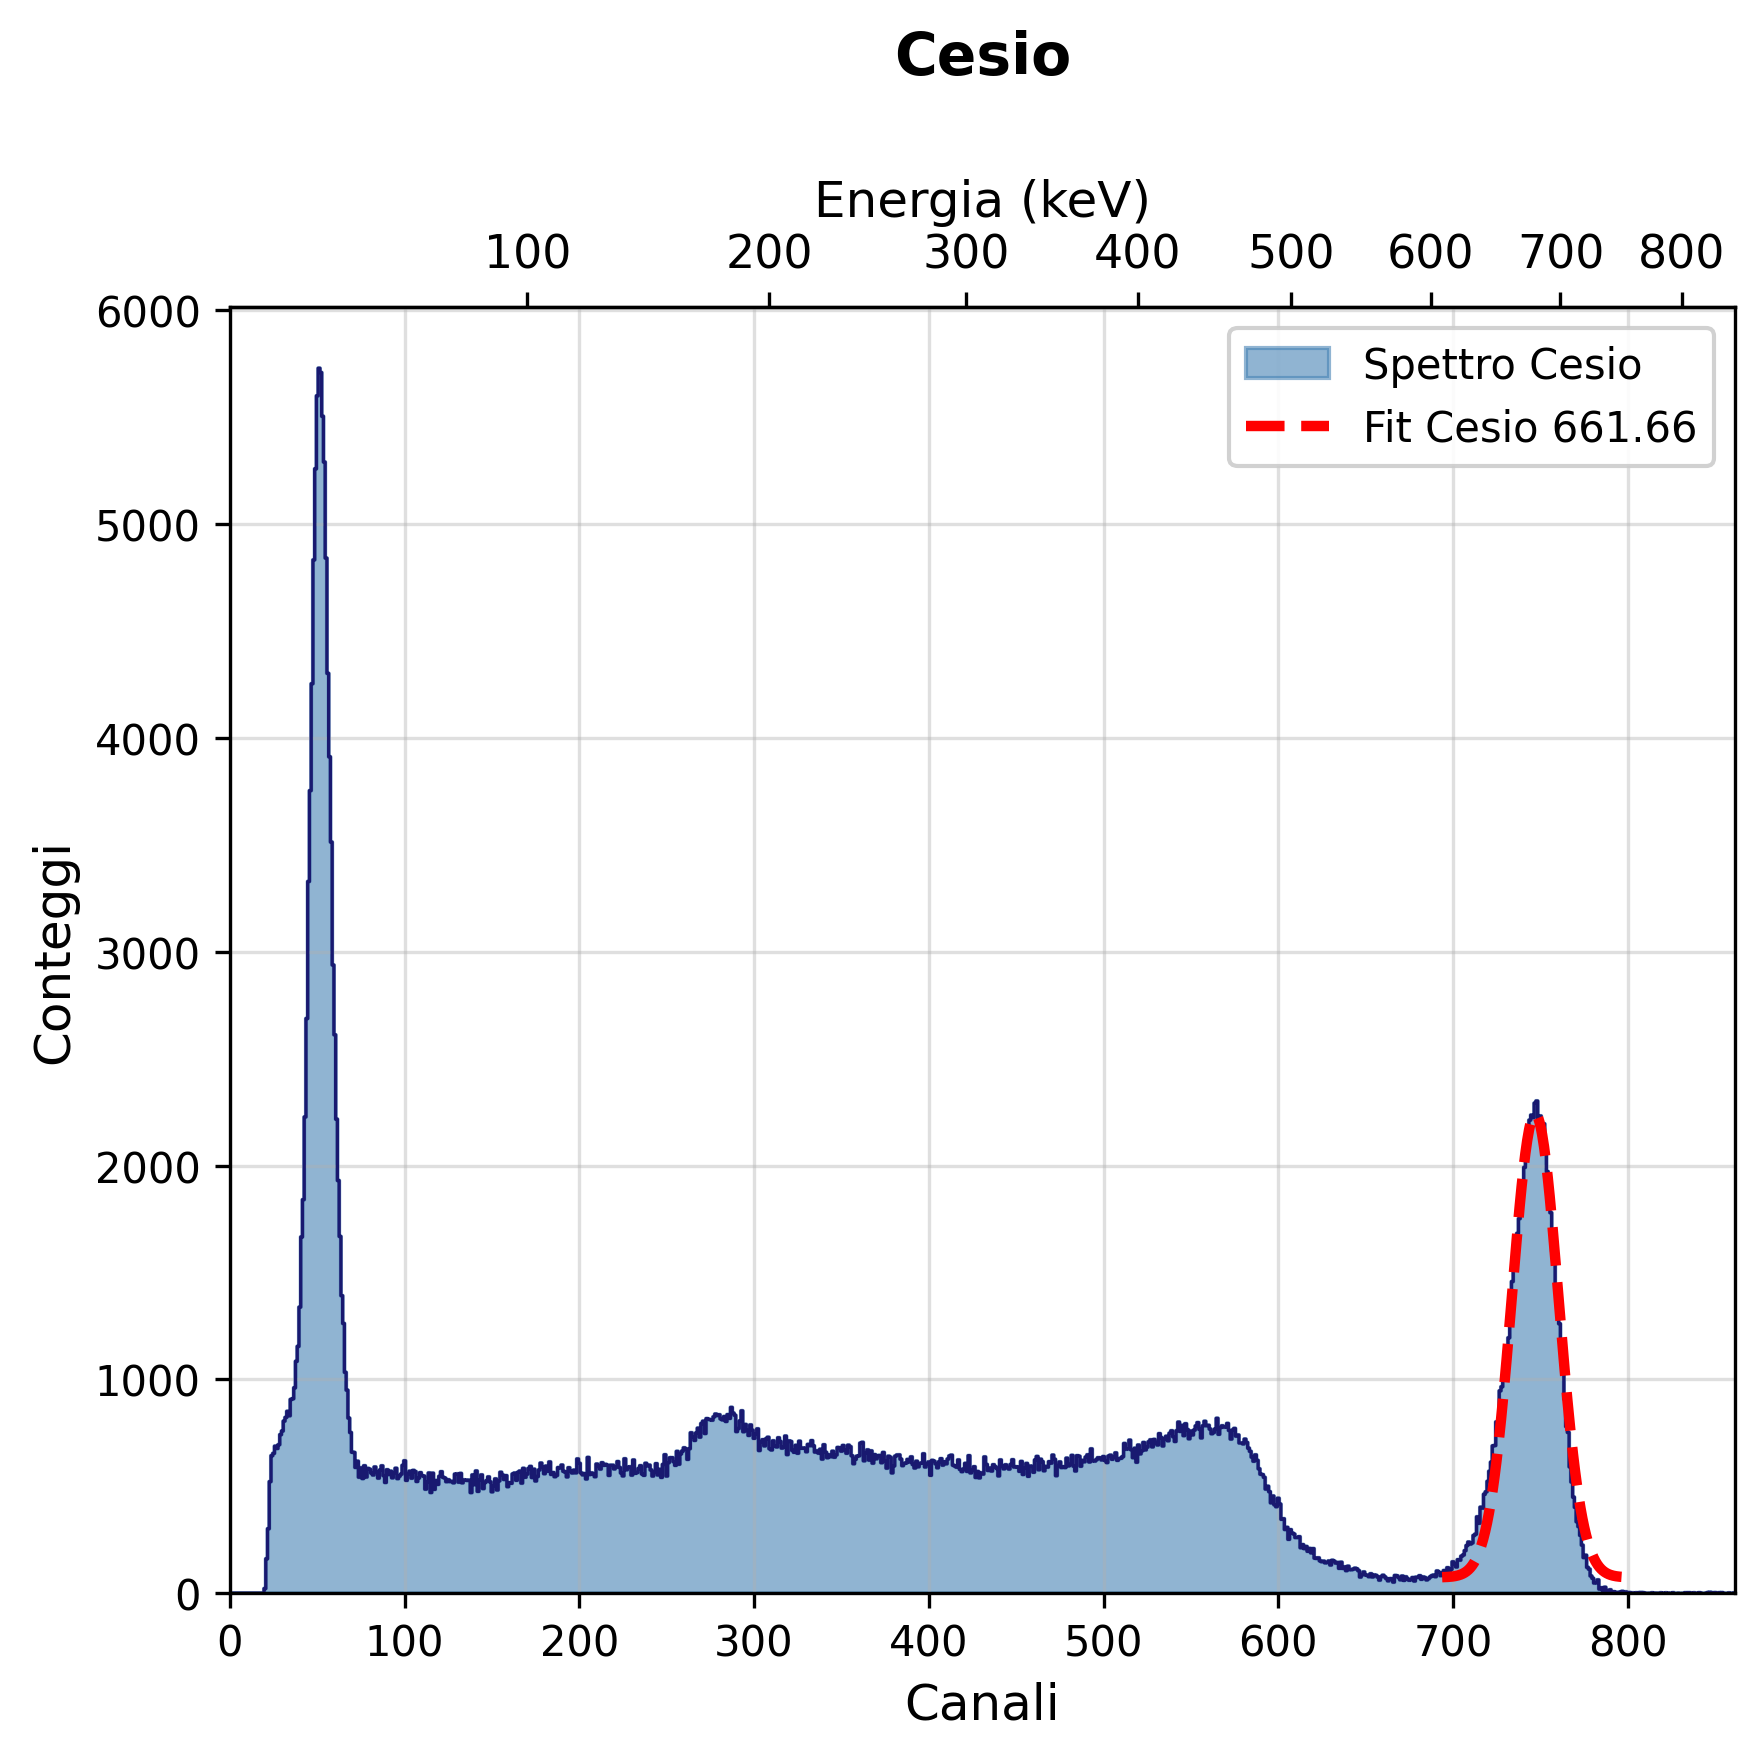
\includegraphics[width=\textwidth]{Spettro_Intero_Calibrato_Cesio.png}
         \caption{Senza blocco di piombo.}
         \label{fig:2a}
     \end{subfigure}
     \begin{subfigure}[b]{0.45\textwidth}
         \centering
         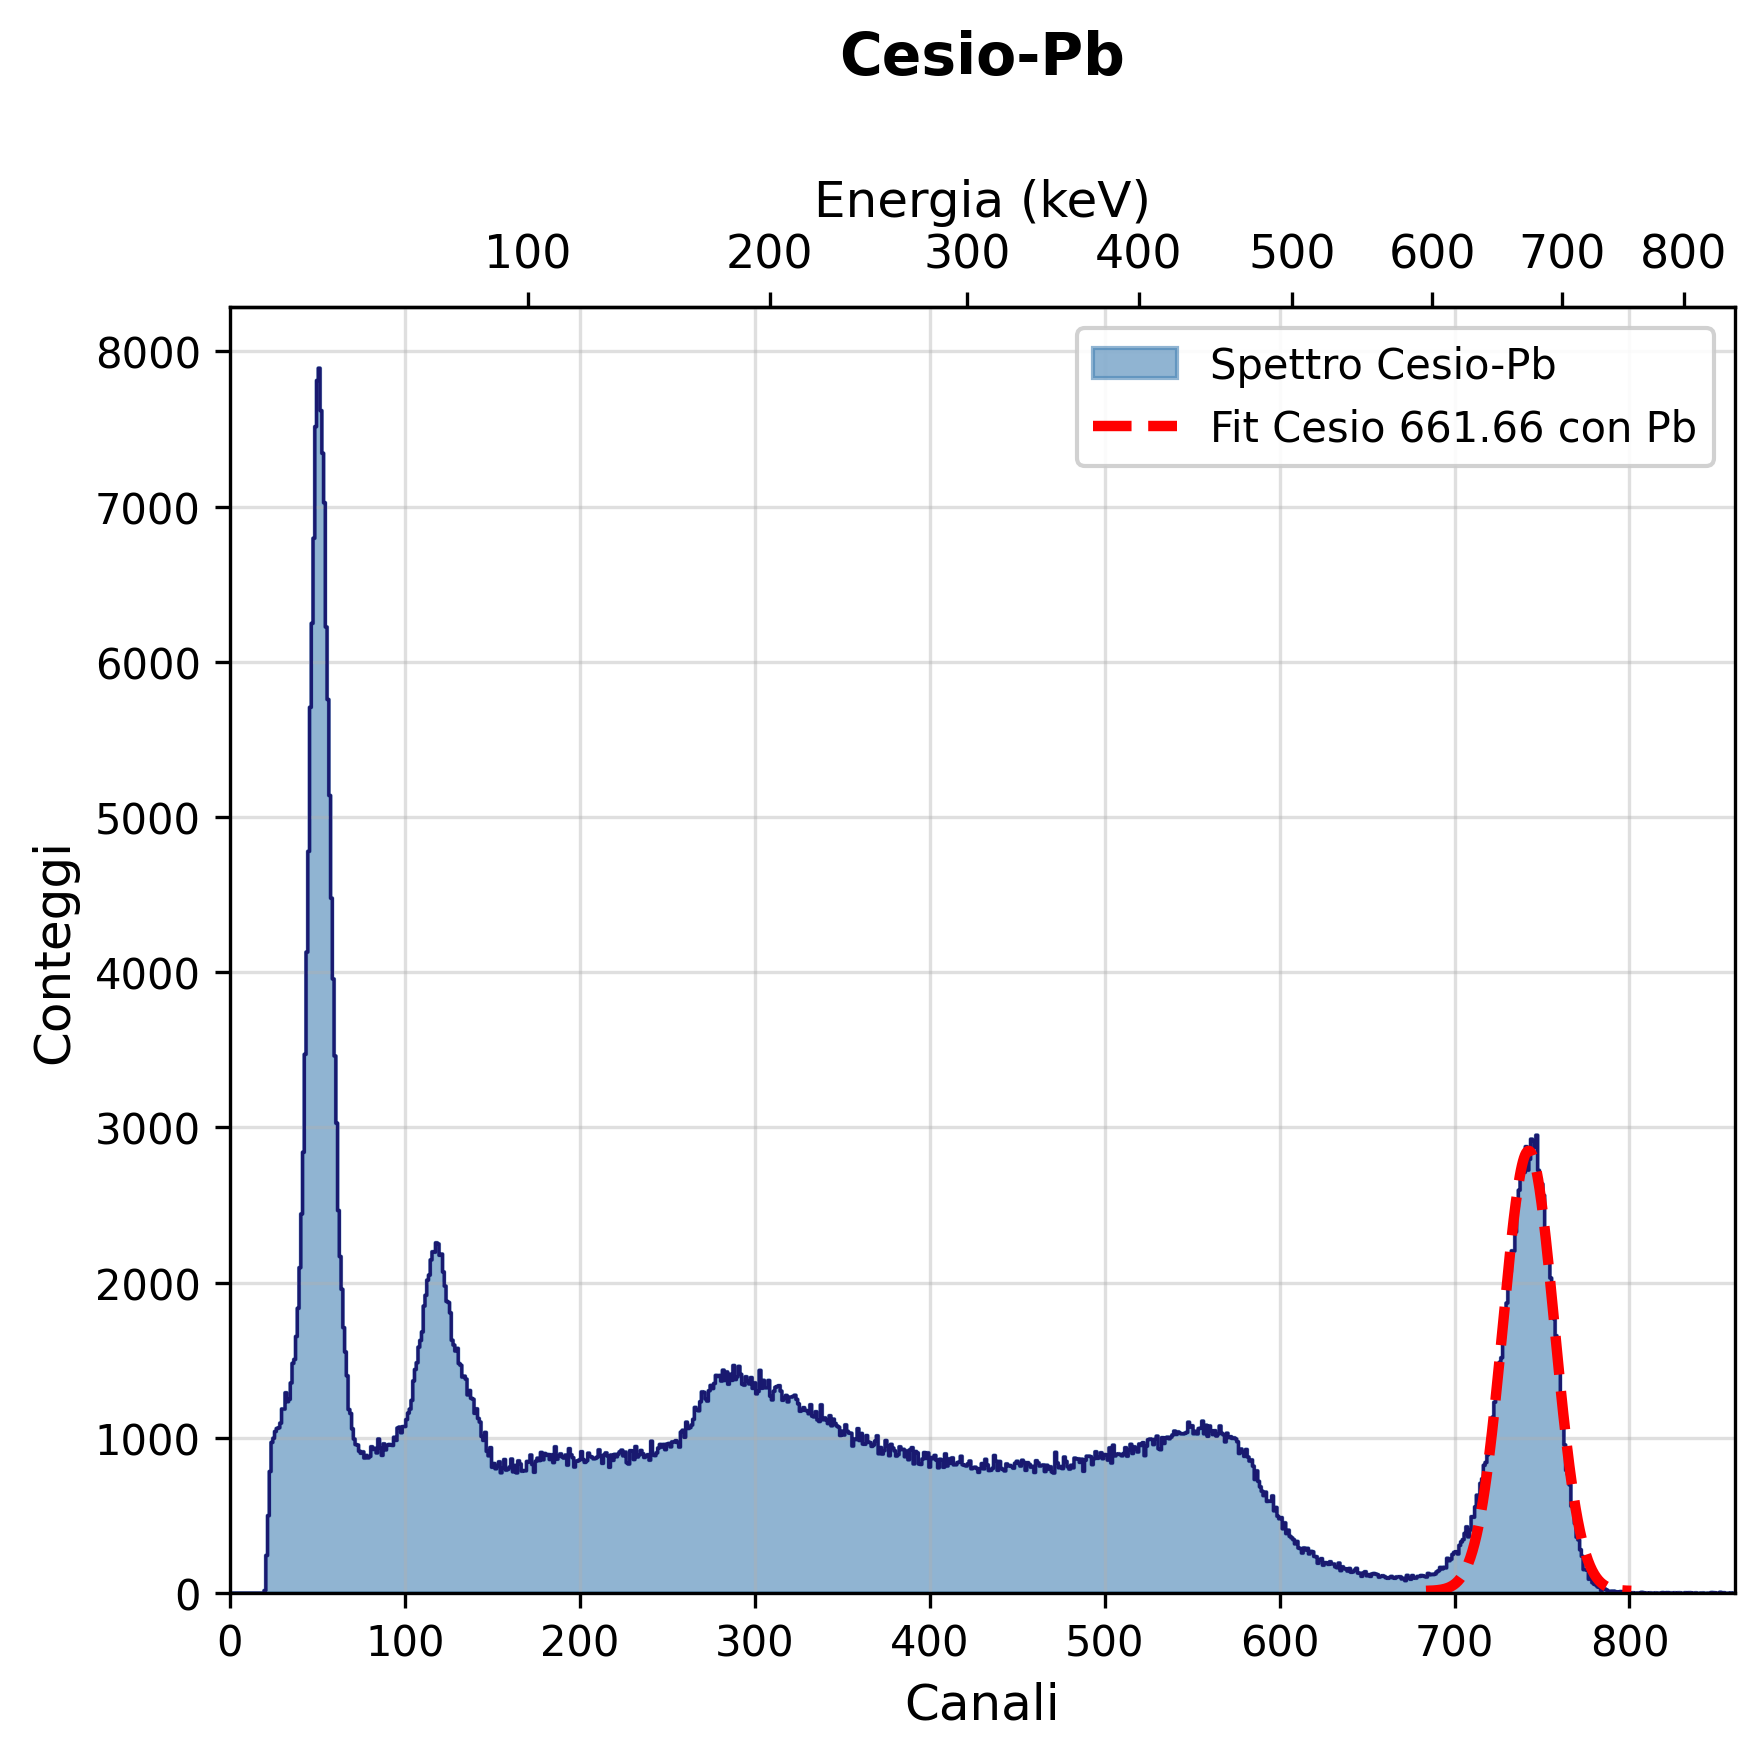
\includegraphics[width=\textwidth]{Spettro_Intero_Calibrato_Cesio-Pb.png}
         \caption{Con blocco di piombo.}
         \label{fig:2b}
     \end{subfigure}
\end{figure}


\subsection{Calibrazione energetica}
Una volta ricavate le posizione dei picchi si è effetuato un fit quadratico delle energie note in funzione dei canali corrispondenti, così da ottenere la curva di calibrazione energetica. La funzione utilizzata per il fit è stata:
\begin{equation}
    E_{teor} = a + b \cdot E_{sper}(ch) + c \cdot E_{sper}^2(ch)
\end{equation}

\begin{figure}[H]
     \centering
     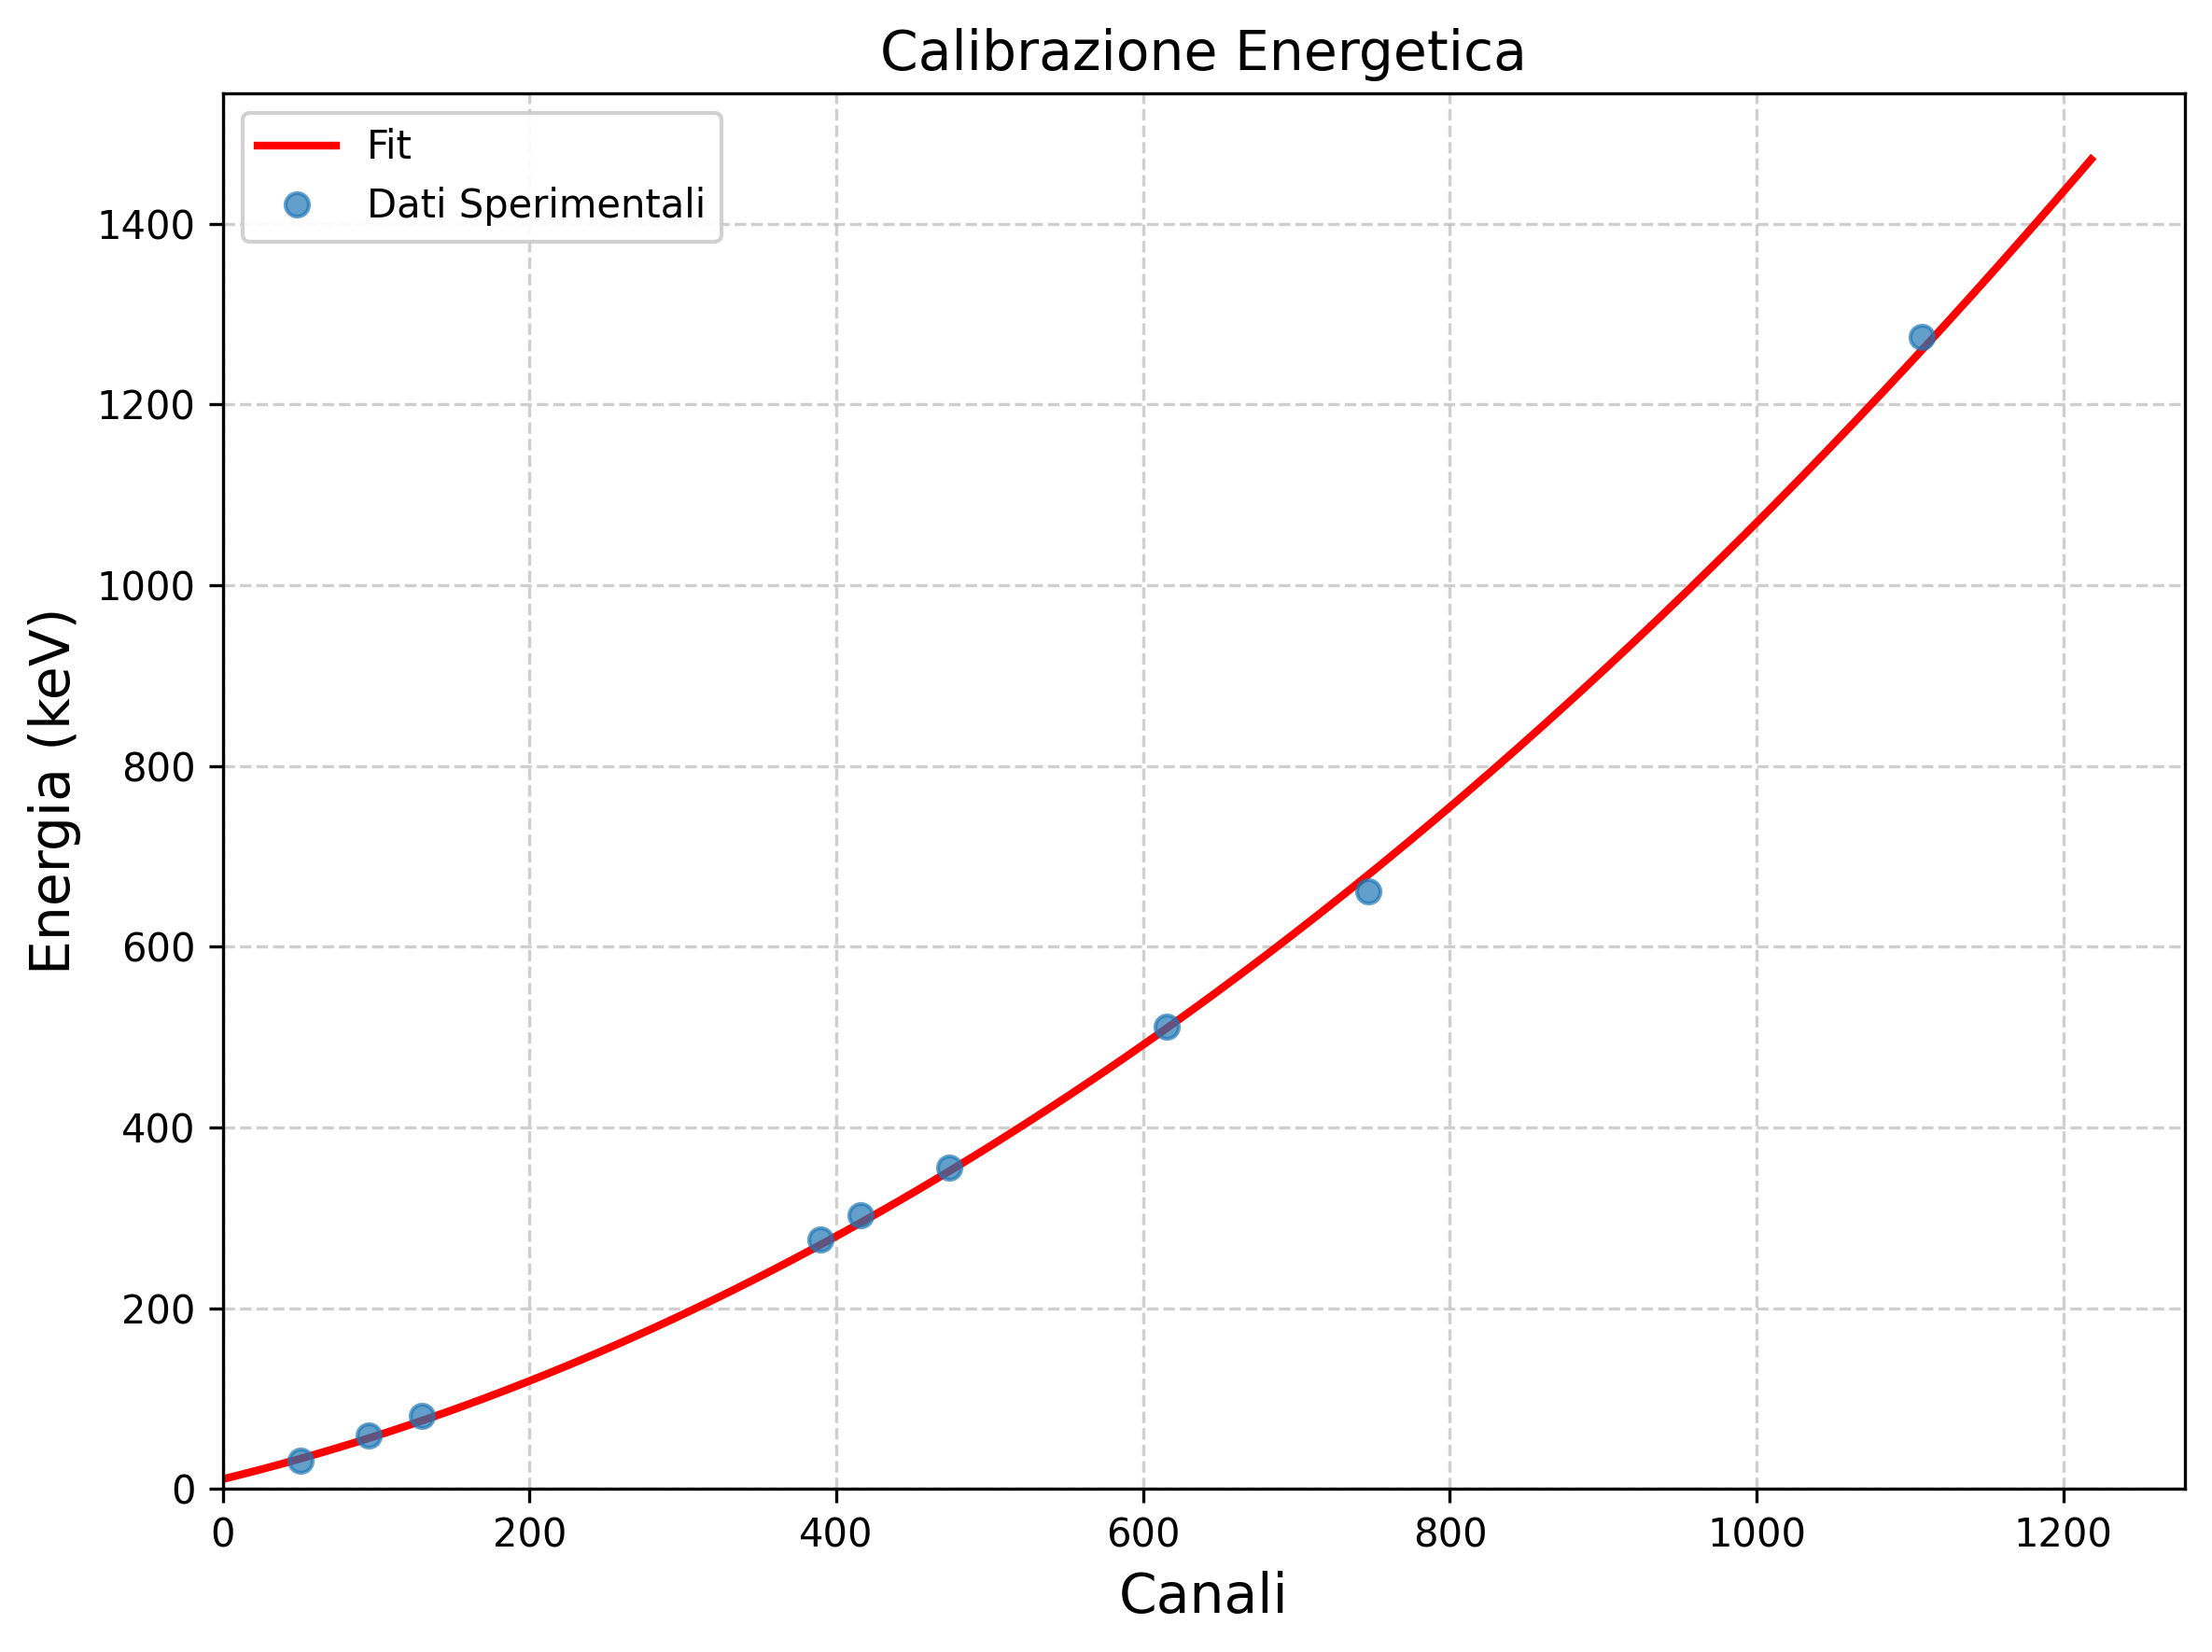
\includegraphics[width=0.8\textwidth]{Fit_finale_calibrazione.png}
     \caption{Curva di calibrazione energetica.}
     \label{fig:3}
\end{figure}

\begin{table}[H]
    \centering
    \begin{tabular}{
        l
        S[table-format=2.4e2]  
        S[table-format=2.4e2]
    }
        \toprule
        {Parametro} & {Valore} & {$\sigma$} \\
        \midrule
        $a$ [\unit{keV}] & 10.77 & 0.06 \\
        $b$ [\unit{\frac{keV}{ch}}] & 0.4146 & 0.0005 \\
        $c$ [\unit{\frac{keV}{ch^2}}] & 6.44e-04 & 5.61e-7 \\
        \bottomrule
    \end{tabular}
    \label{tab:Calibrazione}
\end{table}

\subsection{Risoluzione del rivelatore}
Infine si calcola la risoluzione energetica del rivelatore relativa a ciascun foto-picco tramite le relazioni:

\begin{equation}
    Res[\%] = \frac{FWHM}{E_{peak}}
\end{equation}

\begin{equation}
    Res[\%] = p_0 + \frac{p_1}{\sqrt{E_{peak}}}
\end{equation}

\begin{figure}[H]
     \centering
     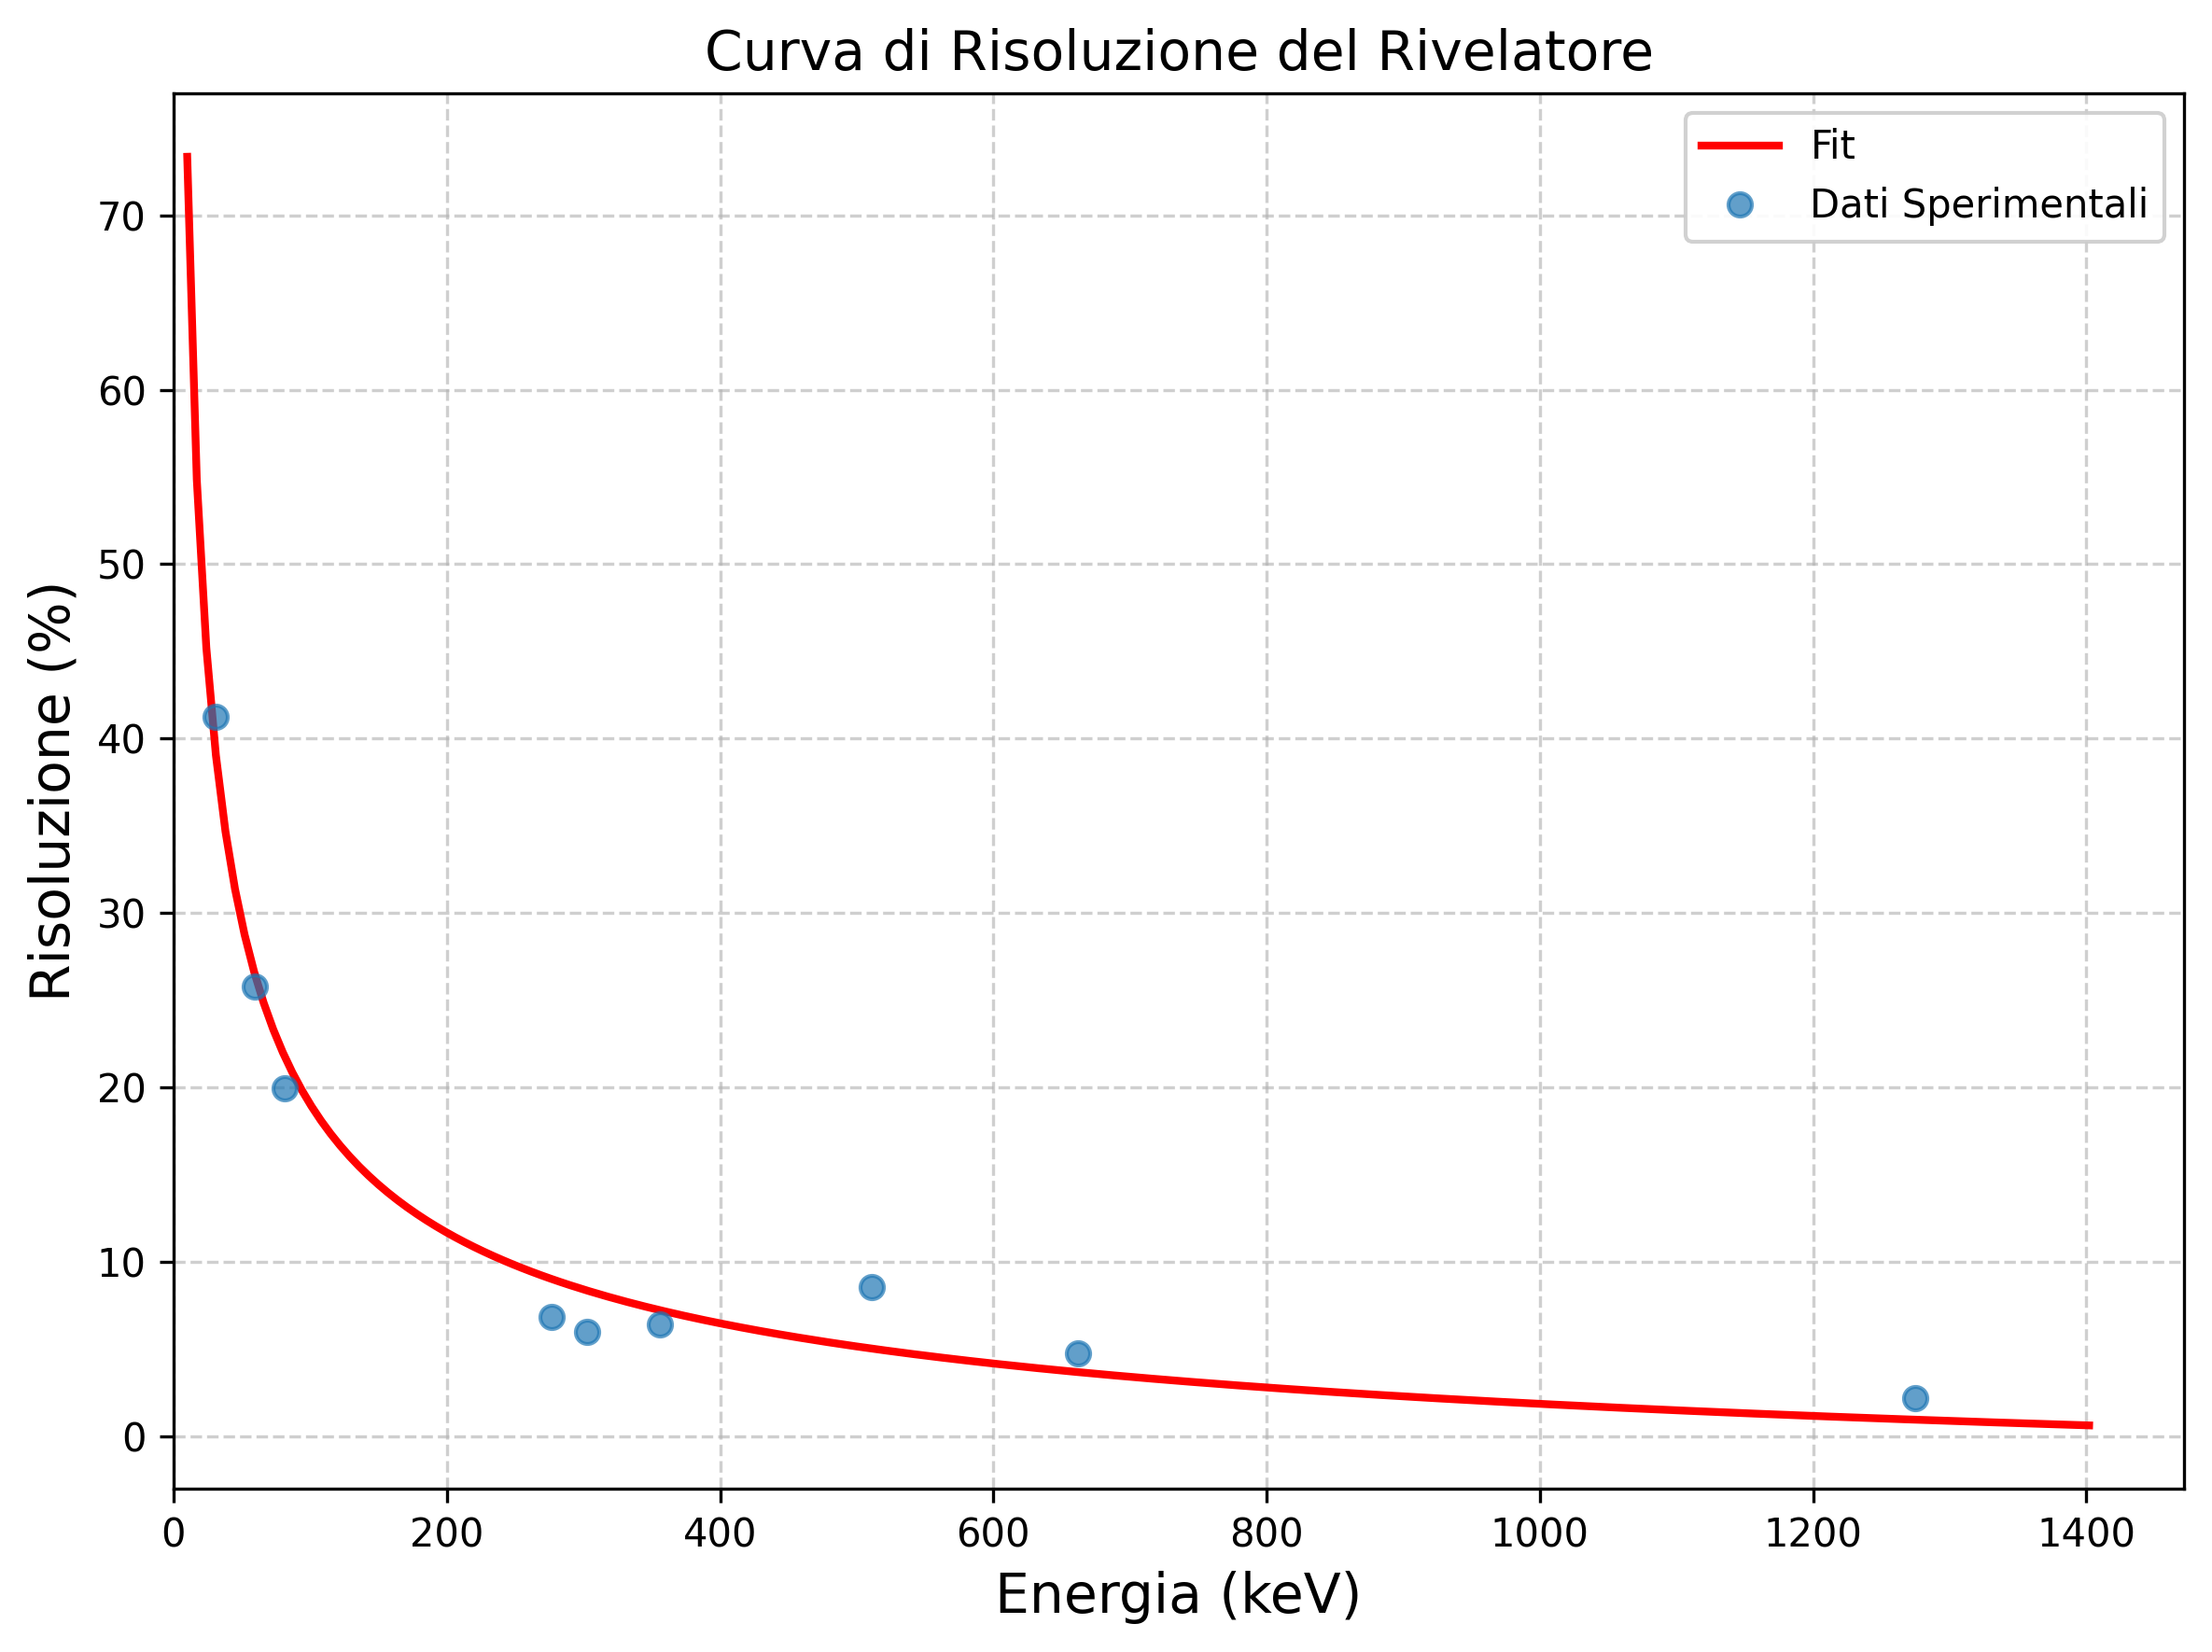
\includegraphics[width=0.8\textwidth]{Fit_finale_risoluzione.png}
     \caption{Risoluzione del rivelatore in funzione dell'energia.}
     \label{fig:4}
\end{figure}

\begin{table}[H]
    \centering
    \begin{tabular}{
        l
        c  
        c
    }
        \toprule
        {Picco} & {Valore Nominale} & {Valore Ottenuto} \\
        \midrule
        \texttt{Cs-137} & 3.5\% & $[3.67 \pm 0.96]$\% \\
        \bottomrule
    \end{tabular}
    \caption{Risoluzione al picco del \texttt{Cs-137}}
    \label{tab:Risoluzione}
\end{table}

% -------------------------------------------------------------------

\section{Conclusioni}
L'analisi degli spettri acquisiti evidenzia, oltre ai fotopicchi principali, ulteriori strutture tipiche dell'interazione radiazione-materia, quali lo spigolo di Compton (Compton edge), il picco di retrodiffusione (backscatter peak) e le emissioni legate ai raggi X caratteristici. In particolare, nello spettro del Cesio-137 acquisito con la schermatura in piombo, si osserva un netto incremento del picco di backscatter e la comparsa di un picco nell'intorno di $80$ \unit{keV}, riconducibile alla radiazione X emessa dal piombo.
Nello spettro di fondo invece si distingue chiaramente un fotopicco isolato nell'intorno dei $1500$ \unit{keV}, probabilmente dovuto all'emissione gamma dovuta al decadimento del Potassio-40, radionuclide che rientra tra i principali responsabili della radiazione ambientale.
Infine dopo la calibrazione energetica si osserva come il valore di risoluzione del rivelatore al fotopicco del Cesio-137 sia compatibile con il valore nominale.
\end{document}